%----------------------------------------------------------------------------------------
% Introduction
%----------------------------------------------------------------------------------------


\section{Introduction} % Add a section title

Inflation is an economic phenomenon in the form of price increase \cite{mankiw:2018}. This is the weighted sum of the different consumer price index (CPI) commodites. In the Philippine setting, rice prices greatly affect the food commodity in the CPI basket. This is mainly because most Filipinos' main food in the table is rice. Thus, an increase in rice prices strongly affects the aggregate inflation. Thus, forecasting rice inflation is significant in inflation outlook.

There have been notable spikes since 1994. In 2008, the sharp increase in inflation is not due to lack if rice stocks since it is obvious in from \textbf{Figure \ref{Stack plots}} that there is an increase in rice stock instead. On the one hand, the short term factors are: (1) temporary export bans and restrictions imlemented by several major and mid-level rice exporters, (2) panic buying by several large rice importers, (3) weather-related problems in specific growing areas, (4) a sharp decline in the value of dollar in fall 2007 and winter 2008, (5) a shift of funds into commodities from shocks and real estate in 2007 and early 2008 that added to price volatility and may have temporarily boosted prices. On the other hand, the long-term factors are: (1) sharply rising incomes in developing Asian countries, (2) very high prices for other foods, (3) extremely high nominal fuel and fertilizer prices, (4) the elimination of excess global rice stocks, (5) negligible yield growth for rice over the past decade, and (6) a massive increase in the production of biofuels in recent years. 
\begin{center}
	\begin{figure} \label{Stack plots}
		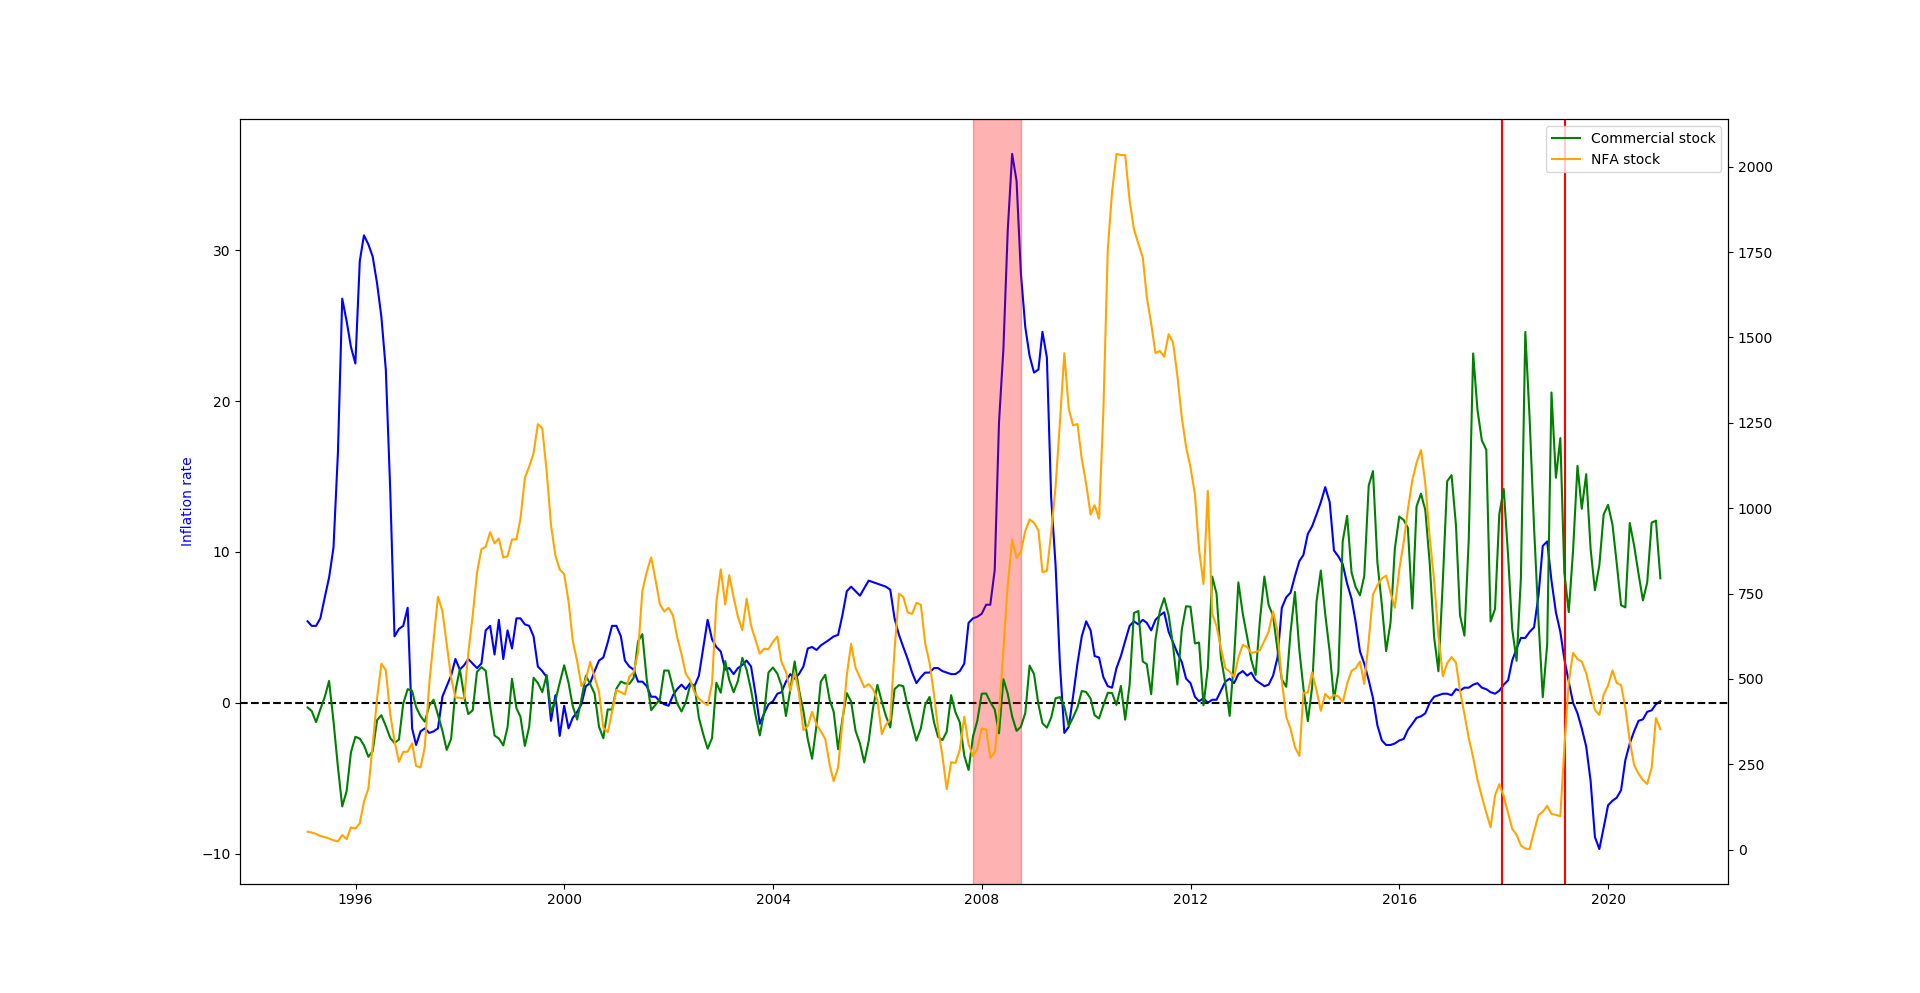
\includegraphics[height=0.6\textwidth]{figure/inf_com_nfa.png}
		\caption{Inflation and rice stock plots.}
	\end{figure} 
\end{center}
